% \begin{minipage}{.45\textwidth}
% \begin{lstlisting}[style=customc, frame=tlrb, caption={Example Code 1}, label=memorySSA-example-1]
% 
% L1: for ( i =0 ; i < 100 ; i++) {
%         S1: A[i] = 0;
%     }
% #pragma omp target enter data map(to:A[0:50], alloc:C[0:100])
% #pragma omp target
% L2: for (i=0; i < 100; i++ ) {
%         S2: t = A[i] ;
%         S3 C[i] = t; 
%     }    
% #pragma omp target exit data map( release:C[0:100])
% L3: for (i=0; i < 100; i++) {
%         S4: print(C[i])
%     }
% \end{lstlisting}
% \end{minipage}
% In this work, we assume that variables
% that have corresponding list items across host and device 
% boundary or across different data environment boundaries 
% on the device need to be updated at the edge of such boundaries. 
% Typically this assumption reflects the practical use-case of the variables. 
OmpSan assumes certain practical use cases, for example, in \autoref{incorrectegs3}, a user would expect the updated 
value of ``B'' after the second data environment on line 12. 
Having said that, a skilled ninja programmer 
may very well expect ``B'' to remain stale, because of his knowledge 
and understanding of the complexities of data mapping rules. 
Our analysis and error/warning reports from this work are 
intended only for the former case.

Here we first outline the key steps of our approach with the algorithm
and exemplify it with a concrete example
to illustrate the algorithm in action.
\vspace{-10pt}
\subsection{Algorithm}
\begin{algorithm}[!htbp]
    \caption{Overview of Data Mapping Analysis}
    \label{dataMapAnalysisAlgo}
    \begin{algorithmic}[1]
        \small 
    \Function{$\textsc{DataMapAnalysis}$}{$Module$}
        \State $MappedArrayVars=\phi$
        \For{$ArrayVar \in MapClauses$}
            \State $MappedArrayVars = MappedArrayVars \cup ArrayVar$
        \EndFor
        \State \texttt{ConstructArraySSA}($Module, MappedArrayVars$)
        \State \texttt{InterpretTargetClauses}($Module, MappedArrayVars$)
        \State \texttt{ValidateDataMap}($MappedArrayVars$)
    \EndFunction
    \Function{$\textsc{ConstructArraySSA}$}{$Module, MappedArrayVars$}
%         \State $MappedArrayVars=\phi$
%         \For{$ArrayVar \in MapClauses$}
%             \State $MappedArrayVars = MappedArrayVars \cup ArrayVar$
%         \EndFor
        \For {$MemoryAccess \in Module$}            
            \State $ArrayVar$ = \texttt{getArrayVar}($MemoryAccess$)
            \If{ 
                $ArrayVar \in MappedArrayVars$ }
            \If { $MemoryAccess  \in OMP\_targetOffload\_Region$}
                \State $targetNode = true$
                \Comment{If Memory Access on device}
            \Else
                \State $targetNode = false$
                \Comment{If Memory Access on host}
            \EndIf
            \State $Range= $ \texttt{SCEVGetMinMax}$(MemoryAccess)$
            \State $underConstruction$= \texttt{GetArraySSA}$(ArrayVar)$
            
            \State \Comment{could be null or incomplete}
            
            \State \texttt{InsertNodeArraySSA}($underConstruction$,$MemoryAccess, targetNode, range$ )
%             \Comment{Incrementally construct, by adding this access}
            \State  \Comment{Incrementally construct, by adding this access}            
            \EndIf 
        \EndFor
        \EndFunction
        \Function{$\textsc{InterpretTargetClauses}$}{$Module, MappedArrayVars$}
        \For {$ArrayVar \in MappedArrayVars$ }
            \State $ArraySSA =$ \texttt{GetArraySSA}($ArrayVar$)
            \For { \textbf{edge}, $(node, Successornode) \in $ ($ArraySSA$) }
%                 \State $node$ = $edge.from$
                \State $nodeIsTarget =$ \texttt{isTargetOffload}($node$)
                
                \State $succIsTarget =$ \texttt{isTargetOffload}($Successornode$)
                \If { $nodeIsTarget \ != succIsTarget$}
                    \State \texttt{RemoveArraySSAEdge(                                                                                                                                                                                                                                                                                                                                                                                                                                                                                                                                                                                                                                                                                                                                                                                                                                                                                                                                                                                                                                                                                                                                                                                                                                                                                                                                                                                                                                                                                                                                                                                                                                                                                                                                                                                                                                                                                                                                                                                                                                                                                                                                                                                                                                                                                                                                                                                          $node$, $Successornode$ )}
                                        
                \EndIf                                                
            \EndFor 
        \EndFor 
        \For {$dataMap   \in dataMapClauses$}
            \State $hostNode$ = \texttt{getHostNode}($dataMap$)
            \State $deviceNode$ = \texttt{getDeviceNode}($dataMap$)
            \State $mapType =$ \texttt{getMapClauseType(}$ dataMap$)
                    \State \Comment{alloc/copyIn/copyOut/persistentIn/persistentOut}
                    \State \texttt{InsertDataMapEdge}($hostNode, deviceNode, 
                    mapType$)
        \EndFor
        \EndFunction
        \Function{$\textsc{ValidateDataMap}$}{$MappedArrayVars$}
        \For {$ArrayVar \in MappedArrayVars$ }
            \State $ArraySSA =$ \texttt{GetArraySSA}($ArrayVar$)
            \For { $memUse  \in $ \texttt{getMemoryUseNodes}($ArraySSA$)}
                \State $useRange$ = $\texttt{getReadRange(memUse)}$
                \State $clobberingAccess =$ \texttt{getClobberingAccess}$(ArraySSA, memUse)$
                \If { \texttt{isPartiallyReachable}($ArraySSA, 
                    clobberingAccess, memUse, useRange$) }
                    \State Report WARNING 
%                     \texttt{Report}($ArraySSA, 
%                     clobberingAccess, memUse, useRange$)                
                \ElsIf { \texttt{isNotReachable}($ArraySSA, 
                    clobberingAccess, memUse$) }
                    \State Report ERROR 
%                     \texttt{Report}($ArraySSA, 
%                     clobberingAccess, memUse, useRange$) 
                \EndIf
            \EndFor
        \EndFor    
        \EndFunction
    \end{algorithmic}
\end{algorithm}
The \autoref{dataMapAnalysisAlgo} shows an overview 
of the data map analysis. Firstly, we 
collect all the array variables used in the various
map clauses in the entire module. 
Then line 5, calls the function \texttt{ConstructArraySSA}, 
which constructs the array ssa for each of the mapped Array variables.
Then, we call the function, \texttt{InterpretTargetClauses}, 
which modifies the Array SSA graph, as per the map semantics of the 
program.
Then finally \texttt{ValidateDataMap} checks the 
reachability on the final graph, to validate 
the map clauses, and generates 
a diagnostic report with the warnings and errors.
% inline all user defined functions, and then use 
% the Memory SSA to construct the memory use-def chains, 
% for every array variable. After step 2, we get a graph for each
% memory array, with an edge from a $MemoryDef$
% or $MemPhi$ to the corresponding $MemoryUse$ or $MemPhi$ for the
% reaching definition relation. 
% Then we use the Scalar Evolution Analysis, to compute 
% the range of locations accessed by every memory reference.
% If the analysis fails to compute the range of locations 
% statically, then we over-approximate it to the 
% maximum size of the array.
% 
% Now we interpret
% the semantics of the \texttt{target} construct, 
% to classify the Memory SSA nodes, as executing on host or device.
% Since the device and host have a separate data environment, 
% they refer to different array variables. So in step 5, we remove the edges between host and device nodes. 
% Now according to the semantics of the \texttt{map} clause, 
% the host variables are mapped to the device variables, and 
% vice-versa. At any program point, when a 
% host variable is mapped to device, 
% we find its corresponding reaching definition, 
% and add a special edge from the host $MemoryDef$ or $MemPhi$, 
% to the $MemoryUse$ or $MemPhi$ on the device. 
% Similarly when mapping a device variable to host variable, 
% we add the edge between the corresponding definition on the device
% to the corresponding use on the host.
% In step 6, we also annotate the edges with the array sections 
% according to the \texttt{map} clause.
% 
% Finally, we report an error for every missing use-def 
% edge in our graph, since it indicates a mismatch
% between the sequential use-def relations and the OpenMp 
% reaching definitions. We report a warning, when an edge indicates
% that the array is partially mapped, and the $MemUse$
% could potentially access locations outside the mapped range.

% \begin{algorithm}
%     \caption{Overview of Data Mapping Analysis}
%     \label{dataMapAnalysisAlgo}
%     \begin{algorithmic}[1]
%         \small 
% %         \Function{$\textsc{DataMapAnalysis}$}{$Module$}
%             
%             \State Construct the Memory SSA for each array variable
% %             \State Dataflow analysis on the 
% %             Use Memory SSA to construct the 
% %             use-def graph for each array variable
%             \State Do scalar evolution analysis 
%             to compute the range of each 
%             memory access            
%             \State Interpret the \texttt{omp target} constructs 
%             and mark the nodes in the SSA graphs as host and device
%             \State Remove the edges from the Memory SSA graph which connect         device nodes with host nodes
%             \State Interpret \texttt{map} clauses to insert edges 
%             in the Memory SSA graph, that correspond to 
%             host-device and device-host memory copies, annotated
%             with array sections 
%             \State For every node in Memory SSA graph, 
%             if the edge from reaching definition is missing, 
%             then Report ERROR
%             \State For every edge connecting host, device nodes, 
%             the array section of the edge must be a subset of 
%             the memory access range of the destination node, 
%             else report it as Warning
% % %             \For{$Memory$ $Access  \in \textsc{Memory SSA}$}
% %                 \If{No Edge between Memory Access and reaching definition}	
% %                     \State Error
% %                 \EndIf
% % %             \EndFor    
%         
% %         \EndFunction
%     \end{algorithmic}
% \end{algorithm}
\begin{figure}[h!]
    \centering
    \begin{subfigure}[b]{0.45\textwidth}
        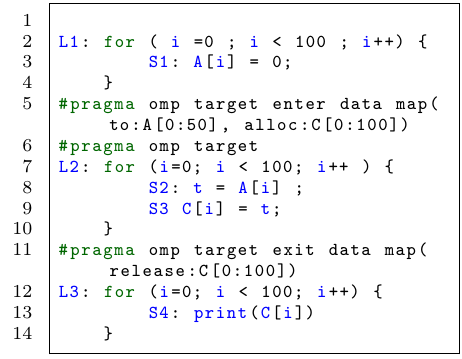
\includegraphics[width=\textwidth]{images/memorySSA-example1.png}
        \caption{Example 1, user Code}
        \label{fig:memorySSA-example1-s4}
    \end{subfigure}
    ~ %add desired spacing between images, e. g. ~, \quad, \qquad, \hfill etc. 
      %(or a blank line to force the subfigure onto a new line)
    \begin{subfigure}[b]{0.5\textwidth}
        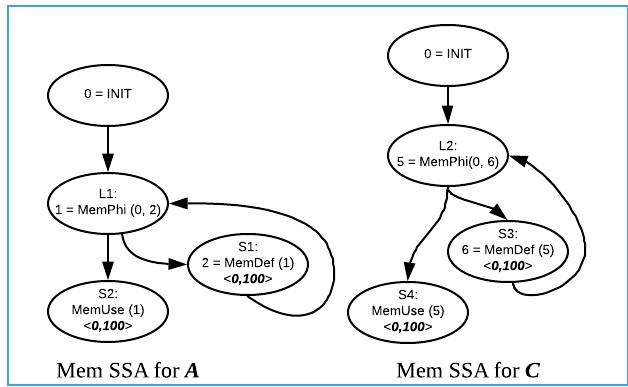
\includegraphics[width=\textwidth]{images/memorySSA-example1-s1.jpg}
        \caption{Memory SSA}
        \label{fig:memorySSA-example1-s1}
    \end{subfigure}
    
    ~ %add desired spacing between images, e. g. ~, \quad, \qquad, \hfill etc. 
    %(or a blank line to force the subfigure onto a new line)
    \begin{subfigure}[b]{0.46\textwidth}
        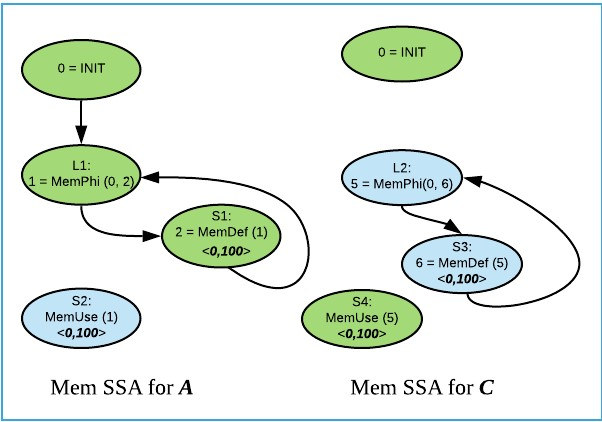
\includegraphics[width=\textwidth]{images/memorySSA-example1-s2.jpg}
        \caption{Classify Host/Device Regions}
        \label{fig:memorySSA-example1-s2}
    \end{subfigure}
    \begin{subfigure}[b]{0.51\textwidth}
        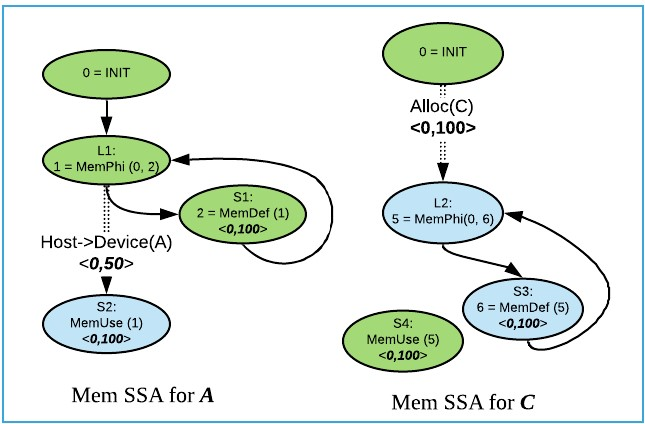
\includegraphics[width=\textwidth]{images/memorySSA-example1-s3.jpg}
        \caption{Host/Device Memory Copies}
        \label{fig:memorySSA-example1-s3}
    \end{subfigure}
    \caption{Data Map Analysis Example 1} 
    \label{fig:memorySSA-example1}
%     \vspace{-100pt}
\end{figure}
\subsubsection{Example 1}
Let us consider the first example \autoref{fig:memorySSA-example1-s4}
to illustrate our approach for analysis of data mapping clauses.
\texttt{ConstructArraySSA} of \autoref{dataMapAnalysisAlgo},  
constructs the memory SSA for arrays ``A'' and ``C'' as shown in \autoref{fig:memorySSA-example1-s1}.
Then, \texttt{InterpretTargetClauses}, removes 
the edges between host and device nodes, as shown in 
\autoref{fig:memorySSA-example1-s2}, where the host is 
colored green and device is blue.
Finally, the loop at line 29 of the function \texttt{InterpretTargetClauses}, 
introduces the host-device/device-host 
memory copy edges, as shown in 
\autoref{fig:memorySSA-example1-s3}. For example
$L1$ is connected to $S2$
with a host-device memory copy for the enter data map 
pragma with \texttt{to}$:A[0:50]$ on line 5. 
Also, we connect \textit{INIT} node with $L2$, 
to account for the \texttt{alloc}:$C[0:100]$, which means 
an uninitialized reaching definition. 

Lastly, \texttt{ValidateDataMap} function, traverses this graph, 
and we can make the following observations,
\begin{itemize}
    \vspace{-5pt}
 \item Error, Node $S4$:$MemUse(5)$ is not reachable from its 
corresponding  
 definition  $L2:5 = MemPhi(0,6)$ 
 \item Warning, Only Partial array section $A[0:50]$, reachable from definition
 $L1: 1 = MemPhi(0,2)$ to $S2:MemUse(1)<0:100>$
\end{itemize}
% These conclusions from our analysis
% are reported to the user along with line numbers from the program, 
\autoref{s5} has several examples of the errors and warnings we report.
% 
% 
% % TODO: Delete following lines 
% verify the correctness of the \textit{map} clauses used by a programmer. 
% \autoref{fig:memorySSA-example1-s4} shows a small program fragment, to illustrate the usage of map clause. \autoref{fig:memorySSA-example1-s1}  shows the memory SSA 
% constructed from the program. We can see the use-def chains for the two memory variables $A$ and $C$ individually. The memory SSA clearly shows the uses and the reaching definitions for the corresponding memory variable. 
% The next step is to interpret the target offload constructs used in the program. 
% The target construct is used to offload a region of code onto a device. \autoref{fig:memorySSA-example1-s2} shows the interpretation of the target construct at line 6 of the program.  
%  The figure uses a color code, 
% to illustrate that the red statements are in the device environment, while the green nodes are the host data environment. 
% In this step, we also remove the memory use-def edges that are across two different environments. So for example, there is no edge between 
% L1 and S2, since the L1 loop is executed on the host, while the S2 is on the device. 
% The last step of our analysis is to interpret the \textit{map} clause used in the program, and add special edges in the memory SSA graph, that corresponds to the host/device memory copy. This step follows the algorithm depicted in \autoref{mapSemantics}. So because of the to map clause on line 5, there is an edge between L1 and S2, which respects the reaching definitions for S2 as per \autoref{fig:memorySSA-example1-s1}. 
% Also, the Alloc edge from init node to L2, signifies the alloc map clause for memory variable $C$.  
% Now, for every Memory Use node, we can validate if there is an edge from its corresponding memory def.
% Otherwise, the \textit{map} clauses were used incorrectly in the user program. 
% So for example, there is still a missing edge between Memory use at statement S4. This means map clauses are wrong and S4 is not reading the appropriate value. 
% \subsubsection{Example 2} 
% For our next example, We modify the \autoref{fig:memorySSA-example1-s4}, with the following map clauses, 
% \begin{verbatim}
%  #pragma omp target enter data map(to:A[0:50], alloc:C[0:100])
%  #pragma omp target exit data map(from:C[0:100])
% \end{verbatim} 
% \autoref{memorySSA-3} shows the SSA graphs 
% for the array ``A'' and ``C''
%  and the final graph after interpreting the map clauses. 
% We report the following warning, after our analysis,
% \begin{itemize}
%  \item Warning, Node $S2$:$MemUse(1)$ uses, $<0,100>$, 
%  which is not a subset of $<0,50>$
% \end{itemize}
% \begin{figure}
% % \hspace*{-80pt}
% 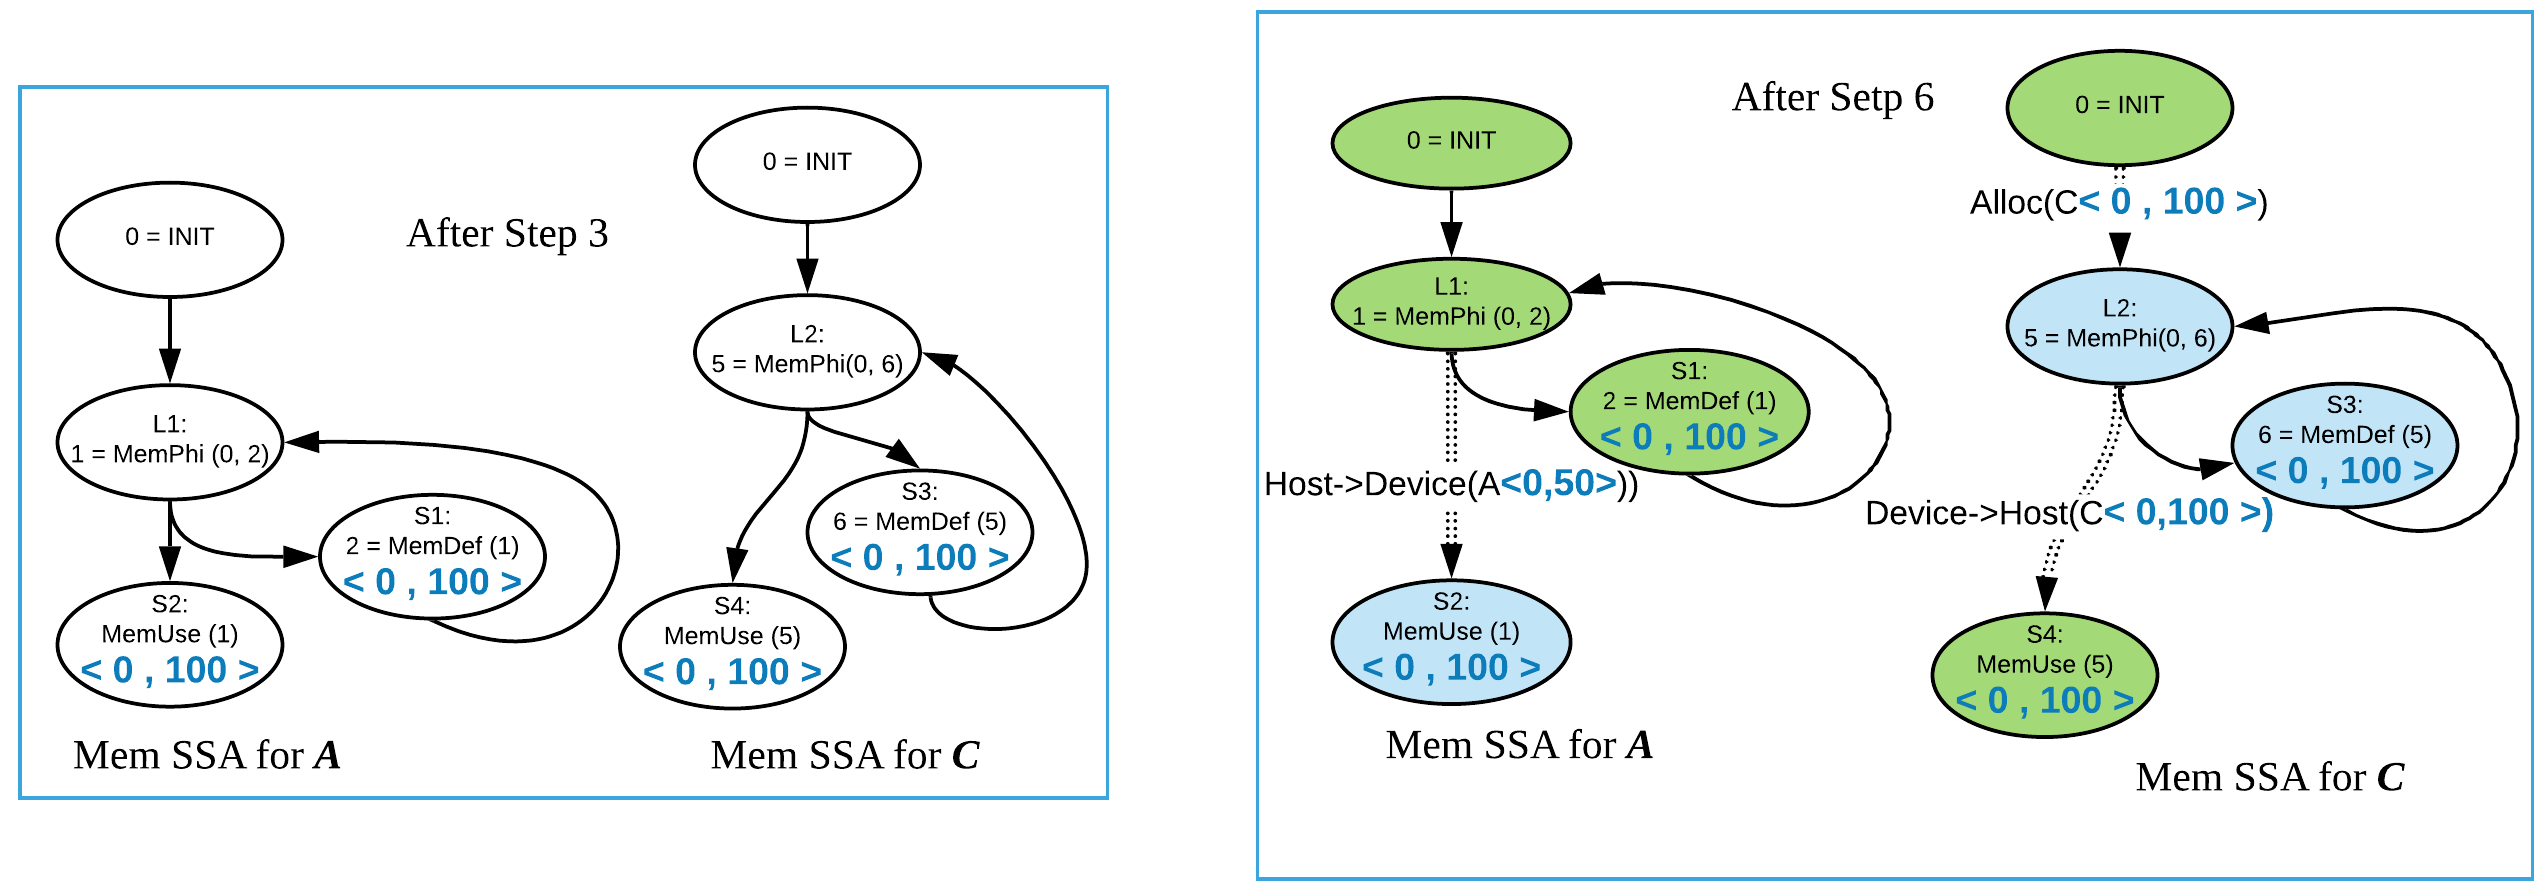
\includegraphics[scale=0.17]{images/memorySSA-3.png}
% \caption{Data Map Analysis Example 2} \label{memorySSA-3}
% \end{figure}
% \subsection{Array Sections}
% \label{SEC:array-sec}
% Next, we look at how to validate the array sections used in the map clause.
% 
% We start with the memory SSA graphs for each memory variable. Each memory def and Memory use corresponds to a statement in the user program. We can analyze the corresponding statement to figure out the index expressions, and the range of values that the expression evaluates to, as shown in \autoref{memorySSA-3}. For example, the index expression at statement S1, has a minimum value of 0 and a maximum value of 100. If the range of the index expression cannot be evaluated statically, then we approximate the range to the size of the memory variable. The size of an array variable is known statically, and the size of dynamically allocated memory variables can be obtained by parsing the corresponding malloc instruction.
% With these annotations, in place, we have a conservative estimate of the range of locations that each memory access refers to. Next step is to interpret the array sections used in the map clauses by the user. It is possible only if the user used compile time constants to specify the array sections in the map clause, as shown in \autoref{memorySSA-3}.
% Each edge between two nodes of different data environments is now annotated with a range. For each such edge, we validate that the corresponding use range is a subset of the range of the edge. Since this analysis is an overapproximation, the violation of this property need not always be an error. Hence we classify this property as a warning.
% \begin{figure}
% \hspace*{-60pt}
% 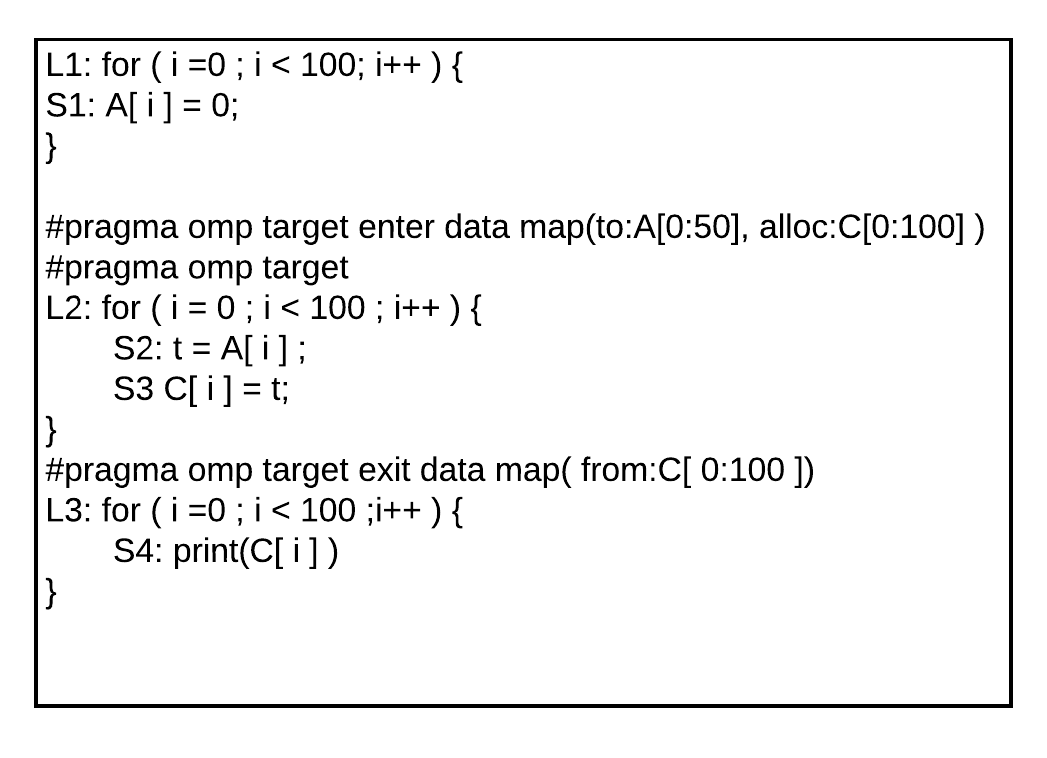
\includegraphics[scale=0.3]{images/memorySSA-3-egs.png}
% \caption{The Algorithm to determine when to insert host-device memory copy} \label{memorySSA-3-egs}
% \end{figure}
